% \begin{savequote}[8cm]
% \textlatin{Neque porro quisquam est qui dolorem ipsum quia dolor sit amet, consectetur, adipisci velit...}

% There is no one who loves pain itself, who seeks after it and wants to have it, simply because it is pain...
%   \qauthor{--- Cicero's \textit{de Finibus Bonorum et Malorum}}
% \end{savequote}

% Proposed old structure (pre-separation into RW and context):
% Global Scholarship Programs
    % A (Recent) History of Global Scholarship Programs
    % The Specific Programs we Work With
    % New and Pressing Selection Problems for these Programs
% Unsolved Problems in Talent Selection
    % Social considerations and the central selection problem
    % Modern Evaluation and the Problem of Generative AI
    % Fair Selection Across Locales
    % The Social and Organisational Value of Diversity
% Existing Quantitative Decision Support Approaches

% New structure is something like:
% Decision Support Tools
% Generative AI Detectors
% Explainable AI
% Quantitative Modelling for Diversity


\chapter{\label{ch:rw}Related Works} 
\minitoc

\section{A (Recent) History of Global Scholarship Programs}
...

\section{Programs we Work With}\label{ssec:programs}
\subsection{Foreword}
We work with two global scholarship and talent investment programs: the Ellison Scholars Program and the Rise Program. Both programs have asked that they not be identified in public facing research, and thus we request that reviewers not share details on Section \ref{ssec:programs} or knowledge contained within. Throughout the remainder of this Thesis, we refer to the Ellison Scholars Program and the Rise Program as Program A and Program B, respectively. However, to provide reviewers with the context and detail required to appropriately evaluate this work, we provide a brief overview of each program in this section.

\subsection{The Rise Program}\label{ssec:rise}
% To-do: I could probably remove detail here
\subsubsection{Program Overview}
Initiated from a $\$1$-billion investment, Schmidt Futures and the Rhodes Trust's Rise program\footnote{https://www.risefortheworld.org/} finds and selects talented and disadvantaged 15-to-17-year-olds from around the world and helps them achieve their full career and service potential. Rise supports selected `winners' and `finalists' with a variety of benefits accessible at different points in their life. We work with Rise from the program's inception in 2021 until 2024. In each of these years, Rise has made a commitment to select up to 100 winners and up to 500 finalists from their pool of applicants. In the four applications cycles between 2021 and 2024, during which time Rise has selected 400 winners and nearly 2000 finalists from hundreds of thousands of started applications.

Rise uses a flexible benefits model, where winners (and, in some cases, finalists) gain access to a variety of potential resources, but utilise only resources they demonstrate need of. For example, applicants who recieve full scholarships to their university may not recieve an academic scholarship from Rise. Program benefits include academic scholarships, educational resources and programs, networking opportunities, and even funding for winner-led startups.\footnote{As academic scholarships comprise a large portion of program benefits, we speak about Rise as a ``scholarship and talent investment'' program throughout. This is our own language, and is intended to further anonymise the program. Similarly, we replace the program-specific term ``winners'' with ``scholars''.}

\subsubsection{The Selection Process}
The program uses a two-stage selection process designed to be accessible to candidates various global and socioeconomic backgrounds. In stage one, applicants submit various application materials asynchronously; Rise selects up to 500 finalists based on the quality of those materials and the program's cohort composition goals. In stage two, finalists engage in one of several ``finalist days'' consisting of various collaborative live activities and an interview; after all finalist days are completed, Rise uses information from both stages to select 100 winners.

\begin{figure}[htbp]
    \centering
    \begin{subfigure}{.45\textwidth}
        \centering
        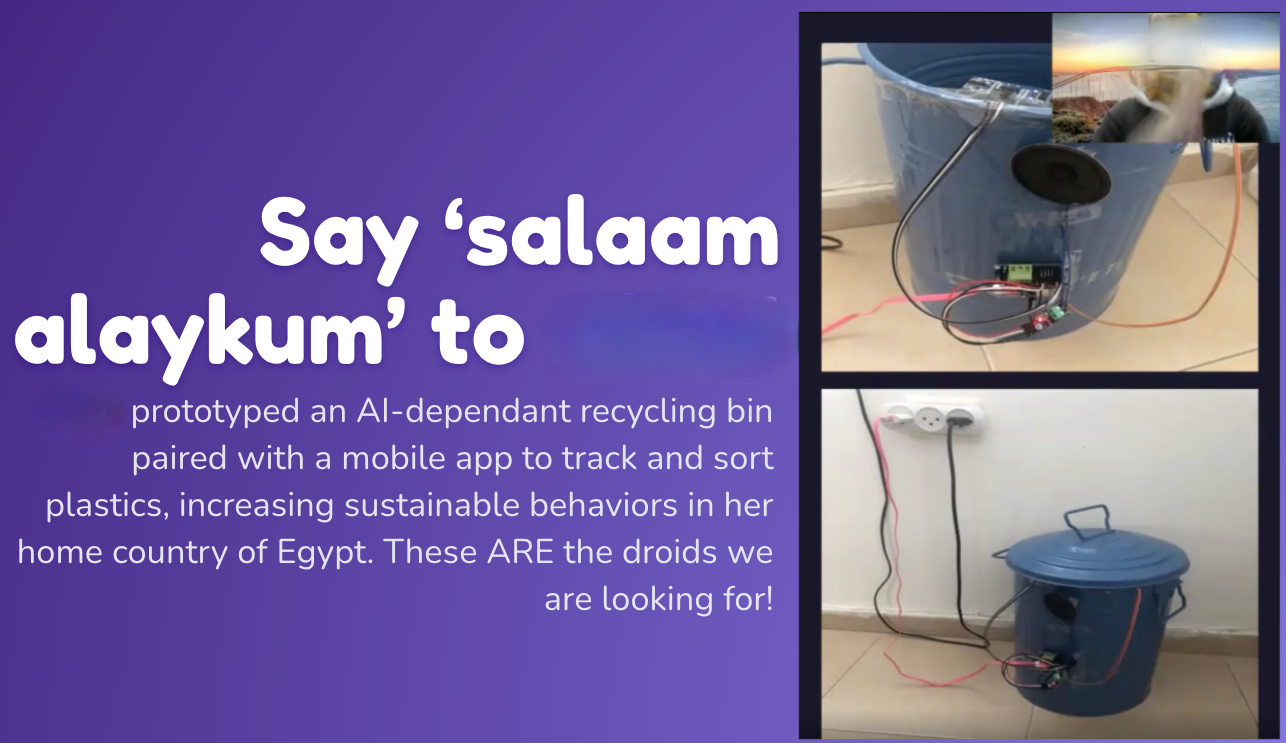
\includegraphics[width=\linewidth]{background/proj1.png}
        \caption{Sample Project 1}
        \label{sfig:can}
    \end{subfigure}
    \hfill
    \vspace{1em}
    \begin{subfigure}{.45\textwidth}
        \centering
        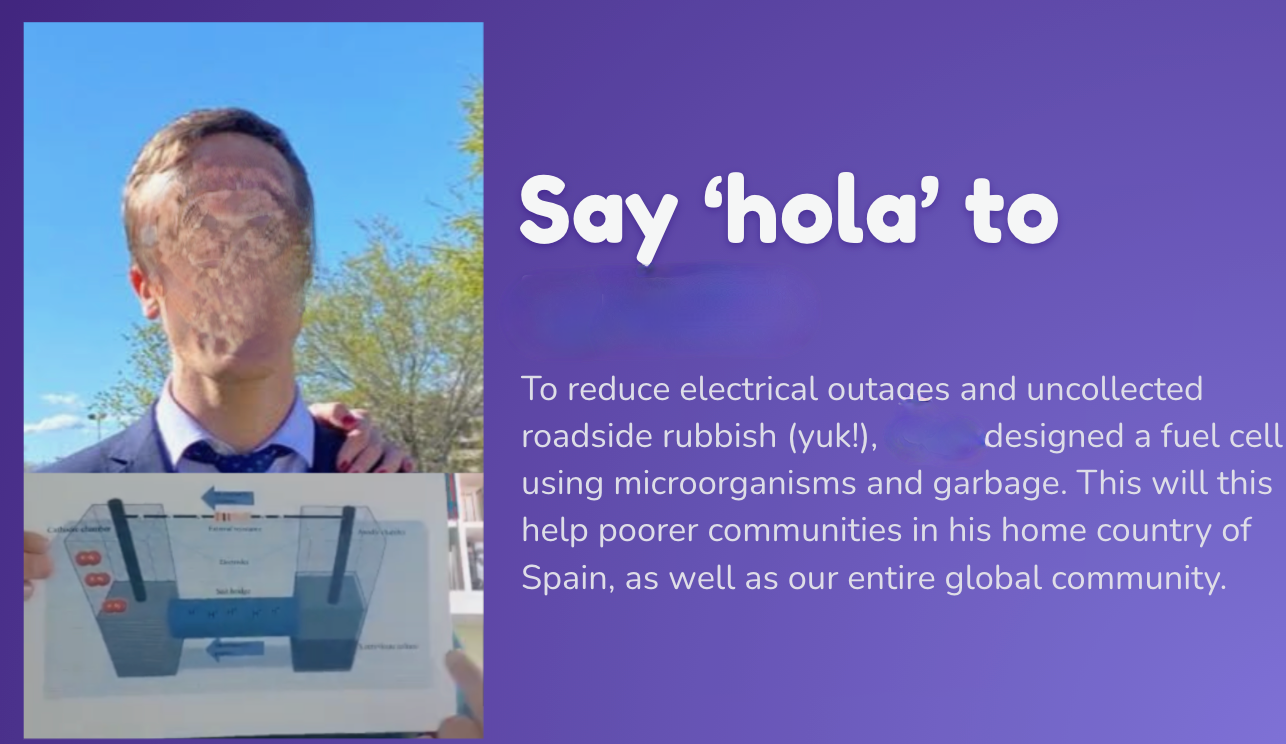
\includegraphics[width=\linewidth]{background/proj2.png}
        \caption{Sample Project 2}
        \label{subfisfigg:cell}
    \end{subfigure}
    \hfill
    \vspace{1em}
    \begin{subfigure}{.45\textwidth}
        \centering
        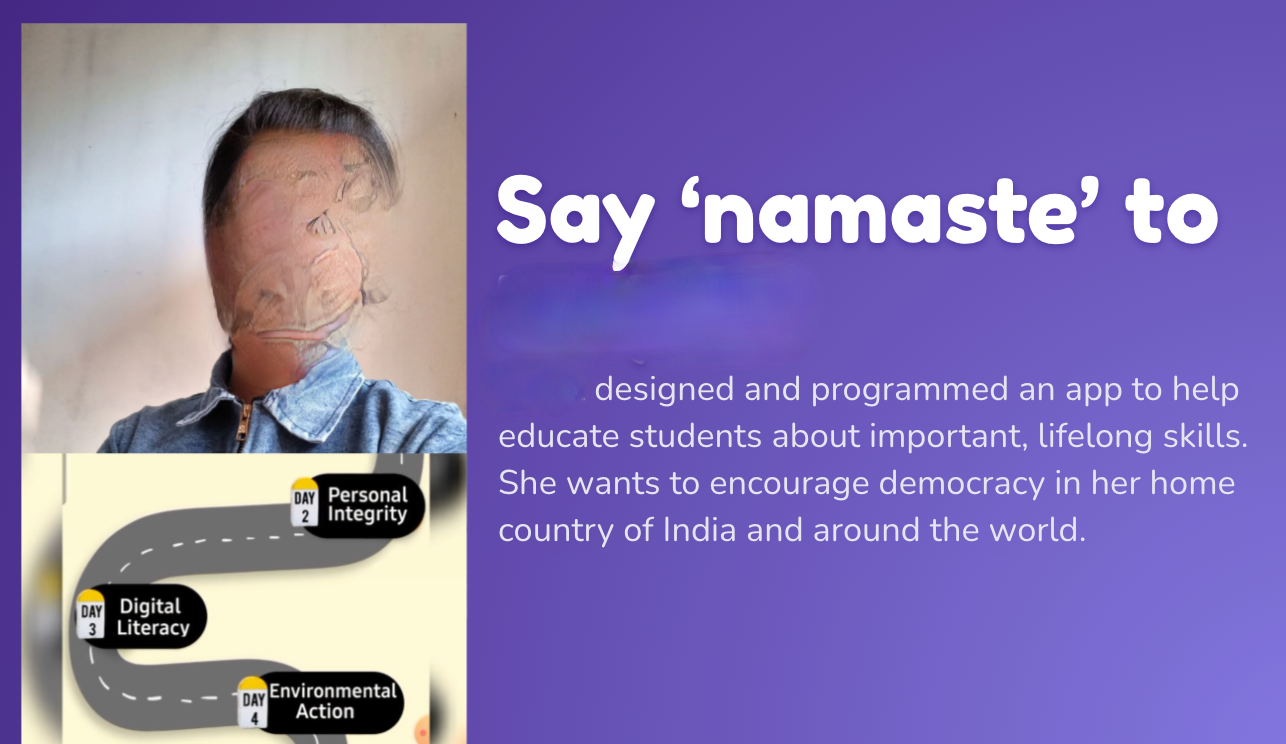
\includegraphics[width=\linewidth]{background/proj3.png} 
        \caption{Sample Project 3}
        \label{sfig:app}
    \end{subfigure}
    \caption{The three panels in this figure depict slides from a program presentation that highlighted three projects that were submitted as part of Rise's 2021 application cycle. Figure \ref{sfig:can} depicts an AI-dependent recycling bin paired with a mobile app to track and sort plastics. Figure \ref{sfig:cell} depicts schematics for a clean fuel cell using microorganisms and garbage. Figure \ref{sfig:app} depicts an app to help education students about the importance of various technical and character skills. Names have been removed and pictures blurred to de-identify program applicants.}
    \label{fig:example_projects}
\end{figure}

Stage one of selection occurs asynchronously (via smartphone, laptop, or, in rare cases, pen and paper) and in two parts. The first part requires applicants to submit an application form with their demographic information and either video or written essays. The first of these two essays explains a real-world problem the applicant wishes to solve, while the second discusses either the ways in which they consider themselves privileged or the challenges they have overcome.\footnote{Refinements to the application process between years all application materials change slightly over time. This change is most dramatic in the case of this second essay, where the focus of the essay changed from an applicant declaration of their own privelege to a description of a challenge the applicant has faced and how they overcame it. Changes appear throughout the application across years; we only detail them where it is relevant to our research.} In the second part, applicants complete a set of digital cognitive assessments and a project showcasing their talent.\footnote{In rare cases, technology or accessibility limitations prevented applicants from completing the cognitive assessment; these applicants were considered on the merits of their submitted materials.} The project showcase is a distinctive part of Rise's selection process whereby particpants: (1) identify a problem they wish to solve, (2) research solutions to that problem, (3) implement those solutions, and (4) reflect on what they learned from the project. Participants submit one essay (video or text) on each of these four stages. Three example projects can be found in Figure \ref{fig:example_projects}. All applicants also submit a short written essay explaining their project and its significance. For an overview of the stage one selection design, see Figure \ref{fig:design}.

\begin{figure}[htbp]
    \centering
    \caption{This figure schematizes the key elements of the talent investment program's data collection and selection process. }
    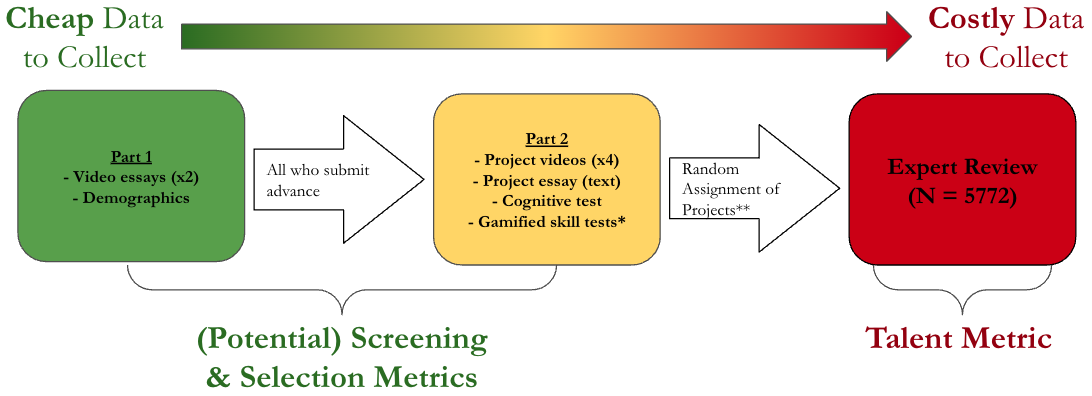
\includegraphics[width=\textwidth,height=\textheight,keepaspectratio]{background/selection_design_schematic.png} 
    \label{fig:design}
\end{figure}

Stage two of selection occurs syncrhonously (though still remotely) in one of several ``finalist days''. The finalist days consist of up to five activities of three types: presentations (where finalists present information about their project), group activities (where finalists collaborate to discuss and solve problems), or interviews (where finalists are interviewed). All activities were judged by a pool of adult `selectors' who assessed finalists according to a rubric. Winner selection decisions were made based both on data collected in stage two and information retained from stage one.

\subsubsection{Program Selection Goals}
- Rise values the 5 traits
- Especially brilliance
- Rise also values diversity

\subsubsection{Data Collection}
Across the application cycle, Rise collects a variety of data from applicants. This data includes traditional merit-based measures – including cognitive tests, written essays, and referrals – as well as non-traditional measures – including peer reviewed video essays, gamified skill tests, and application platform behaviors. Many of these measures are used only for research purposes, and some are tangential to our research on supporting the selection process. We discuss relevant measures here.

% Shorten and rewrite this paragraph (from SPF paper) to suit the thesis.
% Also: the program uses four metrics! Include verbal reasoning!

\paragraph{Cognitive Assessments}
% In all three cycles, applicants took an intelligence test based on the International Cognitive Assessment Resource (ICAR) \cite{condon2014international, subotic2020psychometric}. The full ICAR test is intended to be an accessible and easy-to-understand test that yields a psychometrically validated measure of IQ. Because the program is international, they use only the three item types that are not heavily reliant on English language knowledge: Cube Rotation, Number Sequence, and Matrix Reasoning. All three item types are best described using language from the \hyperlink{https://icar-project.org/types/index.html}{ICAR website}: the Cube Rotation items "present participants with cube renderings and ask participants to identify which of the response choices is a possible rotation of the target stimuli", the Number Sequence items ask participants to "fill in one or two numbers that follow in the sequence", and the Matrix Reasoning items "contain stimuli that are... 3x3 arrays of geometric shapes with one of the nine shapes missing" (similar to those used in Raven's Progressive Matrices) and participants "are instructed to identify which of six geometric shapes presented as response choices will best complete the stimuli". Depictions of each item type are shown in Figure \ref{fig:icar_items}. 

% ICAR scores are generated from estimation of a Bayesian generalized linear item response model following \textcite{burkner2021bayesian}. In particular, define an indicator of whether person $p$'s answer to item $i$ is correct as $\psi_{pi}$. $\psi_{pi}$ is modeled as being determined by a respondent effect -- interpreted as a person $p$'s cognitive ability $\theta_p$ -- and an item effect -- interpreted as the item $i$'s difficulty $\xi_i$. The model also includes and additional \emph{discrimination} parameter $\alpha_i$ which allows items to vary in how well they differentiate high ability vs. low ability respondents. Altogether, this means 

% \begin{equation}
% \psi_{pi} = f\big(\alpha_i(\theta_p + \xi_i)\big). \nonumber
% \end{equation}

% Following the literature, the link function $f(\cdot)$ is logistic, which makes it a general linear model. In particular, we have

% \begin{equation}
% \psi_{pi} = \frac{\mathbb{e}^{\big(\alpha_i(\theta_p + \xi_i)\big)}}{1 + e^{\big(\alpha_i(\theta_p + \xi_i)\big)}}, \nonumber
% \end{equation}

% Which is estimated using Bayesian GLM via \textbf{brms} \textbf{R} package. Bayesian methods were employed to allow the program to utilize prior knowledge from ICAR scoring on meaningfully different, but larger samples. The cognitive ability score assigned to each applicant $p$ for analysis in this paper is the percentile of the median of the posterior distribution of $\theta_p$.

% In addition to ICAR, the program also collected an ability measure from a gamified skills test called Roomworld. Roomworld is intended to measure intelligence and creativity in a way that is fun, novel, and not dependent on culture-specific knowledge. In each level, applicants are challenged to move through the grid using the arrow keys to get the yellow icon to a gift icon. Shapes within the grid serve as different obstacles and mechanisms for navigating the level. How each obstacle and mechanism work are not explained to the player, as part of the test is about discovering how they work. For an example level of the game, see Figure \ref{fig:roomworld_instance}. Multidimensional data from the game are collected and aggregated to give players a percentile score.\footnote{Roomworld was created and scored by an external partner to the program and the specific scoring algorithm was not shared with the authors of this paper.}

\paragraph{Peer Review}
Stage one applicant essays were judged by two types of human evaluators: other applicants (peers) and adults with some expertise on the project topics (experts). Though \textcite{citation needed} provide some evidence for peer review as a measurement of aptitude, peer review was (and remains) experimental, and Rise treated it as such. To collect peer reviews, each applicant was assigned to review 20 of each essay submitted. Each review consisted of Likert scale judgements designed to measure: intelligence, perseverance, empathy, integrity, sense of calling, and impact on the applicant (see Table \ref{tab:rise_measure_details} for details of measurement).

\paragraph{Expert Review} 
Experts, on the other hand, were only asked to assess applicant project essays. Each reviewer was assigned a number of projects proportional to their capacity to review. Like peers, experts were asked to review different elements of the project, using Likert scales to gauge how effective the project was at accomplishing what the applicant intended and how impressive the project was relative to other projects in this field (see Table \ref{tab:rise_measure_details} for details of measurement). 

\paragraph{Finalist Day Activities}
The finalist day activities were assessed by selectors through a mix of qualitative and quantitative measures. Each activity was scored on a rubric, and the scores were aggregated to create a final score for each finalist on each activity type. Additionally, selectors were given an option to provide specific qualitative feedback on applicants.

\subsection{The Ellison Scholars Program}\label{ssec:ellison}
\subsubsection{Program Overview}
Funded and adminsitered by the Ellison Institute of Technology, The Ellison Scholars Program\footnote{https://eit.org/ellisonscholars/} is a global scholarship program that seeks to develop global technology innovators and leaders by finding and supporting talented people passionate about solving humanity’s most serious problems as they study at the University of Oxford and solve global problems through innovation. The program seeks to select at least twenty scholars each year beginning in 2025.

As the Ellison Scholarship's innagural cohort has yet to be selected, program benefits have yet to be dispersed. However, the program has committed to providing scholars with an academic scholarship to the University of Oxford and paid internships. These internships, as well as the program as a whole, are organised around four humane endeavours: (1) Health and Medical Science, (2) Food Security and Sustainable Agriculture, (3) Climate Change and Clean Energy, and (4) Government Innovation and Era of Artificial Intelligence.

\subsection{The Selection Process}
The Ellison Scholarship employs a three-stage selection process. In stage one, applicants submit various application materials asynchronously; the program selects semi-finalists based on the quality of those materials and the program's cohort composition goals. In stage two, semi-finalists apply to the University of Oxford, and the University handles their own internal selection process; program applicants who recieve Oxford scholarships are dubbed Finalists. In stage three, finalists engage in a series of synchronous activities before final decisions are made by the program's board. 

In stage one of selection, applicants submit: their demographic information; selections for humane endeavour, Oxford course, and preferred project; their education record; a list of achievements; and four written essays speaking to their suitability for the program. These essays speak to the applicant's alignment to their chosen humane endeavour, alignemnt to their chosen course at Oxford, and their particular skills and archetype. After submitting this application, all applicants are invited to take a cognitive assessment assessing convergent and divergent reasoning.

In stage two, semi-finalists apply to the University of Oxford; in stage three, finalists engage in a series of synchronous activities before final decisions are made by the program's board. As the Ellison Scholars program is still selecting their innagural cohort, neither stage two nor stage three have been enacted. Thus, we omit details on them here. 

\subsubsection{Program Selection Goals}
- the Ellison Scholars selects around institute projects and humane endeavours
- While many members of the team are sympathetic to demographic diversity, more cognitive definitions are more gemane

\subsubsection{Data Collection}
The Ellison institute collects and constructs a number of different aptitude measurements of applicants. This is primarily traditional merit-based measures, e.g., cognitive tests, written essays, or academic transcripts. Additionally, the program constructs a number of more experimental measures from gathered data. We discuss relevant measures here.

\paragraph{Cognitive Assessments} 
Much like the Rise program, the Ellison Scholarship uses a cognitive assessment based on the International Cognitive Assessment Resource (ICAR) \cite{condon2014international, subotic2020psychometric}. Though the details of implementation differ, both programs use the same four item types and same scoring algorithm.

Additionally, the Ellison Scholarship relies on a divergent thinking assesment based on Guildford's Alternative Uses Task (AUT) \cite{citation needed}. % To-do: more on the aut, including scoring methodology and a sample item.

\paragraph{AI-driven Assessment of Essays}
% To-do: fill this out

\paragraph{Expert Assessment of Applications}



% To-do: transform this into a subsection about applicaitons of xAI as decision support tools
\section{Interpretable Artificial Intelligence}
\subsection{Types of IAI Publications}

The field of IAI can, broadly, be divided into four main bodies of research: reviews, methods, notions, and evaluations \cite{vilone_explainable_2020}. Review articles are either systematic investigations or literature reviews. Method articles introduce new explanation methods. Notion articles focus on defining notions or concepts related to explainability. Evaluation articles evaluate existing notions or paradigms.

\subsubsection{Review Articles}
Review articles offer meta-commentary on other articles listed below. A review article is so-characterised because its primary contribution is one of aggregation. Thus, a review article might also be a method, notion, or evaluation article, so long as it primarily draws from these articles. This paper is, primarily, a review article.

\subsubsection{Method Articles}
In most method articles, the task of explanation is taken to be fairly well-defined, and the research questions deal in how to most effectively generate that explanation. 

Consider two particular method articles: SHAP explanations, introduced by \textcite{lundberg_unified_2017}, and counterfactual explanations, introduced by \textcite{wachter_counterfactual_2017}. In both papers, we see heavy treatment of the mathematical properties of the explanation algorithm introduced. However, we see relatively light treatment of what the authors take to be a good explanation or proposed use cases for the novel methods. These concepts are instead the domain of notion articles.

\subsubsection{Notion Articles}
Where method articles deal with individual methods, notion articles deal with theory underlying a variety of methods. For example, \textcite{miller_explanation_2017} discussion of the importance of principles of explanation from the social sciences is a notion article.

\subsubsection{Evaluation Articles}
Evaluation articles consider which notions and methods are best-suited to produce the best explanations. Evaluations of method articles, in particular, often compare them to notions introduced elsewhere, and where critiques are found, they are often critiques that the method fails to meet a standard set by the notion.

For the two method articles discussed above, we present two evaluation articles: \textcite{kumar_problems_2020} evaluation of the SHAP method, and \textcite{barocas_hidden_2020} evaluation of counterfactual explanations. Both articles rely on similar notions regarding the purpose of explanations, and critique the methods for failing to adhere to a notion. For instance, \textcite{barocas_hidden_2020} assume that counterfactual explanations are given to provide users actionable information. Similarly, \textcite{kumar_problems_2020} argue that SHAP cannot be used to inform users' actions.

\subsection{A Taxonomy of IAI Methods}
AI model explanations can broadly be categorised into two subgroups: intrinsically interpretable models and post-hoc explanations \cite{molnar_interpretable_2019}. Though intrinsically interpretable models offer explanations and are meaningfully classed as forms of “interpretable AI”, they do not make use of the major developments in “explainable AI” \cite{molnar_interpretable_2019}, since they are already interpretable.

Post-hoc methods can be further separated into global methods, which explain entire models, and local methods, which explain individual decisions \cite{molnar_interpretable_2019}. When assessing explanation methods, one can distinguish between local tests and global tests of model explanations \cite{molnar_interpretable_2019}. Local tests concentrate on the impact of the explanations at the level of a single prediction, global tests focus on the impact of explanations on overall model trust.

Rather than delineating between intrinsic and post-hoc or global and local, we could instead delineate by output type \cite{friedrich_taxonomy_2011}. Some interpretability devices offer feature importance statistics. Others offer explanations by contrast to another datapoint. Yet others offer rules that guide decision-making in regard to an individual case case.

\subsection{Use Case}
Consider the following potential use cases for xAI methods: to evaluate whether the AI is operating as intended, to examine an AI for bias and unfairness, to provide recourse, to provide a rule that would guarantee equality. This list is not exhaustive, and yet, even for these three use cases, explanations that satisfy some will not satisfy others \cite{natarajan_trust_2023}.

\subsection{Theories of Explanation}
In deciding which type of explanation will best suit a particular use case, we must consider the theory of explanation that underlies the explanation, and the desiderata that that theory demands of its explanations.

\textcite{miller_explanation_2017} summarises key findings from Social Sciences related to explanation. \textcite{miller_explanation_2017} works from a causal theory of explanation; he outlines and examines the theory, noting challenges to it, but does not consider a rejection of the theory. According to the theory, explanations are sought in response to counterfactual cases, i.e. the question asked is not of the form "Why \textit{P}" but rather "Why \textit{P} instead of \textit{Q}" \cite{miller_explanation_2017}. Such counterfactual theories of causality all argue that cause is a matter of what would have happened if the cause had not happened. Though they disagree on precisely how to model these counterfactual cases, many leading philosophical theories of causality agree that causality is best understood in terms of counterfactuals. Hume modeled these counterfactuals in terms of causes and events: in actuality, cause $C$ caused event $E$ to occur; but if cause $C'$ had replaced cause $C$, $E$ would not have occurred. We can call this sort of counterfactual a cause-counterfactual \cite{miller_explanation_2017}. Under this conception, explanations should present cause-counterfactuals as clearly as possible.

\textcite{miller_explanation_2017} also argues that explanations should be contrastive and selective. Contrastive explanations make use of counterfactuals, but these counterfactuals are not cause-counterfactuals. Instead, they are event-counterfactuals. In other words, contrastive explanations consider alternative events $E'$, and explain the data $E$ in relation to $E'$. Selective explanations, on the other hand, are ones that do not consist of a complete cause, but rather select one or two causes from the complete cause. 

\textcite{miller_explanation_2017} presents a powerful application of a theory of explanation to the field of xAI. However, causal theories of explanation are far from the only type of explanatory theories. Indeed, as we noted above with numerical evidence, there are theories of explanation who's desiderata contradict those of \textcite{miller_explanation_2017}'s causal theory \cite{woodward_scientific_2021}. 

In what follows, I present \textcite{woodward_scientific_2021}'s theory, the statistical relevance model of explanation. The statistical relevance theory rests heavily on the notion of statistical relevance. For events $A$, $B$, and $C$, we say $C$ is statistically relevant to $B$ in $A$ if and only if $P(B | A \land C) \neq P(B | A)$. I.e., an explanation is a member $C_i$ of a homogeneous partition $C$ of properties: that is, a set of properties that are exclusive and exhaustive of $A$, where there are no statistically relevant properties $D$ to $B$ in $A \land C_i$. The explanation also consists of $P(B | A)$, the probability $P(B | A \land C_i)$ of each cell withing the partition, and which of the $C_i$ contains the desired point to be explained, $x$ \cite{woodward_scientific_2021}.

On both accounts , explanations have an explainer and an explainee. Explanations in everyday use are an interaction. Unlike most modern algorithmic explanation methods, an explanation given by a human is often given in the form of a conversation. Thus, it obeys the rules of communication using language. In other words, these explanations are social. We may therefore apply theories governing social interactions, such as \textcite{Grice_1975}'s conversational maxims, to explanations \cite{miller_explanation_2017}.

\textcite{Grice_1975}'s four categories of conversational maxims are: quality, quantity, relation, and manner. That is, the quality of information conveyed in a cooperative conversation should be high (information should be likely and justifiable). The quantity of information should be neither too little nor too much. The information should be related to the conversation. The information should be conveyed in an appropriate manner. Note that the quantity bounds overlap quite heavily with selectivity.

\subsection{Trust}
Another important notion related to xAI is trust. Indeed, much of the xAI literature suggests that the purpose of xAI is to increase trust in AI. This is apparent from the titles of canonical papers in the field, such as \textcite{ribeiro_why_2016} and \textcite{pieters_explanation_2011}. So what does it mean to trust an AI system? A basic philosophical analysis of what trust consists in (in the general, non-algorithmic sense) is as follows: $A$ trusts $B$ if and only if $A$ believes that $B$ will act in $A$'s best interest, and $A$ accepts vulnerability to $B$'s actions \cite{jacovi_formalizing_2021}. Moreover, trust often does not have a blanket scope; typically, $A$ will trust $B$ regarding some particular actions or motivations.

An important distinction here can be drawn between whether someone or something is trusted and whether that trust is warranted; i.e. it is worthy of trust \cite{hardin_trust_2002}. In the context of AI, according to \textcite{jacovi_formalizing_2021}, we should only ever trust AI systems to fulfil their contracts, but some AI systems are not worthy of even this trust. Ideally, trust in a system should relate directly to that system's trustworthiness – we should place trust in any system when it warrants trust, but should not place unwarranted trust in any system. The problem of appropriately calibrating trust, however, is yet unsolved.

There are many methods that aim to calibrate trust in an AI algorithm. We could give some access to the patterns that distinguish correct and incorrect cases. The better some end-user is able to distinguish these, the better they know when they can trust the model to be correct. Knowledge of the performance of a model grants access to the patterns distinguishing correct and incorrect cases. Facts about the bias of the model grant access as well, as does information about the performance of the model on a subset of data. Explanations can be seen as one way of imparting such information. Because of this, algorithm explanations allow explainees to determine when an algorithm is trustworthy. 

\subsection{Relevant Evaluations of XAI}
There is a growing body of studies that empirically evaluate xAI methods. In some cases, an xAI method is evaluated not with human subject experiments but rather with some formally defined proxy for interpretability \cite{doshi-velez_towards_2017}. However, most evaluations involve humans using an AI system to perform some task, and the effect of an xAI method on task performance is measured.  For our purposes, namely the measurement of end-user trust and reliance, we need to measure lay people using a system in a simplified but realistic task.

It should also be noted that there is no standard evaluation or set of benchmarks explainability methods are judged by \cite{doshi-velez_towards_2017}. Indeed, though there are proposed methods for evaluating attribution-based explanations and model-based explanations, there are none for evaluating example-based explanations \cite{markus_role_2021}. As a result, there exist a variety of study designs, conditions, and variables measured by human-centred evaluation papers. We list some such studies here.

\textcite{ford_play_2020} run a study where they examine the impact of post-hoc explanations-by-example and error-rates on people's perceptions of a black-box classifier. They show that case-based explanations lead participants to perceive miss-classifications as more correct. In the case of their study, a case-based explanation is a series of three important data points in the training of the model (in other words, an “influential instances” explanation). They also show that classifiers with higher error rates lead participants to perceive the models as less trustworthy. They show participants a series of machine classifications of the MNIST dataset, where the model either correctly labels the data or commits an alternate labelling error. They then task the participants with rating correctness and reasonableness of each classification on a 5-point scale. Finally, at the end, the participants filled out global correctness and reasonableness, alongside global trust forms. The design was a 2x3 design, with explanations present or absent, and three accuracy levels. Participants report miss-classifications as being more correct when given a case-based explanation. They did not find significant findings for reasonableness, trust, or satisfaction across explanation-present or explanation-absent conditions. They use a MANOVA design to account for differences across conditions, but use a between-subjects design \cite{ford_play_2020}. 

\textcite{jacobs_how_2021} run a study in the medical diagnosis context, where participants are given a vignette of a patient and, in the experiment condition, a recommended treatment list and explanation. Participants were asked to make an antidepressant treatment selection, to rate their confidence, and to indicate the utility of the model on their decision (it appears on a 5-point scale). The study had statistically significant results only with respect to accuracy (measured as an average of 0s and 1s), not confidence or perceived utility. In the accuracy case, this indicated that an algorithmically generated treatment list, when wrong, would mislead the participants and lower their accuracy. In the confidence and utility cases, this would indicate either that accuracy is affected, but not confidence or utility, or that the Likert scale measurement method used in Jacobs et al.'s study is a weaker measurement tool than the accuracy. Furthermore, these findings are not isolated to the explanation. Rather, Jacobs et al. consider the recommendation and the explanation together. For example, they find that feature-based explanations, paired with incorrect recommendations, lowered accuracy compared to the baseline condition (no recommendation) \cite{jacobs_how_2021}. 

\textcite{bansal_does_2021} perform another similar study, looking at human-AI cooperation in a context where they have comparable performance. They use sentiment classification as their task. Furthermore, they measure effects with a variety of explanations. They find that explanations inspire increased trust in AI systems regardless of the correctness of the model. As explanation, they use a highlighting of the top predicted sentiment classes, alongside a highlighting of important words. Finally, they test expert-generated explanations to serve as an upper bound, as they found that humans were often confused when machine explanations made little sense. They note that explanations make the user more likely to have high accuracy when the AI is correct, but more likely to have low accuracy when the AI is incorrect. This would indicate that AI recommendations with explanations are capable of fostering mistrust, as they foster both overtrust and under trust \cite{bansal_does_2021}.

\textcite{mohseni_trust_nodate} measure user trust in an AI fake news detection system over time. They design a study in which users are shown true and fake news articles. The users are asked at three different points (each one additional third through the study) what their perceived accuracy of the explainable AI system is. They had three different conditions, segmented by type of explanation. There was a baseline condition with no explanation and two xAI conditions. They show that the user trust can be clustered into five profiles: consistent overtrust, consistent under trust, consistent trust, trust gains continually, and trust decreases continually. They show that more participants from the no explanation and attribute explanation conditions were consistently gaining trust, and that more participants from the attention explanation condition overshot their second perceived accuracy measurement \cite{mohseni_trust_nodate}.

\section{Open Problems in Diverse, Equitable, and Inclusive Talent Identification}
We highlight several open problems in TI that touch on concerns of DEI. To begin with, we define DEI alongside related concepts such as JEDI, EDI, DEIB, and IDEA. Then we spotlight the potential equity challenges posed by the integration of DSTs into TI workflows. In particular, we note that any bias and fairness issues built into a DST will create bias and fairness issues for the corresponding TI workflow. However, we note that problems of bias and fairness in TI exist even in the absence of DSTs. We move on to discuss fairness issues posed by applicant use of Generative AI. Finally, we note that TI professionals consistently struggle to balance selecting talented individuals with constructing a diverse cohort and note the implications for equity that this struggle brings.  

\subsection{Bias}
\subsubsection{The Problem of Bias}
We can define the problem of bias as the liability of systems to exhibit different behaviour on groups segregated across a “special” partition. “Special” here refers to partitions across protected classes, or partitions across which we would expect a system to perform equally. For example, gender and race are usually special partitions in the context of talent identification, but academic ability and teachability are not. 

To illustrate the issue of bias in AI systems, we turn to \textcite{mattu_how_nodate}'s analysis of the COMPAS system. The COMPAS system was an expert-system used to predict recidivism of criminals in the US. When defendants accused of crimes were booked in jail, they responded to a COMPAS questionnaire. These answers were then fed into the COMPAS software to produce predictions of the “Risk of Recidivism” and “Risk of Violent Recidivism.” These predictions were used, among other things, to determine if a defendant could be set bail (as likelihood of reoffence is a significant factor in the setting of bail). When \textcite{mattu_how_nodate} analysed the COMPAS tool's predictions relative to actual recidivism rates, they found that the recidivism predictions had roughly equal accuracy for White and Black defendants, but that, when errors were made, these errors acted in very different directions. That is, the Black defendants were more likely to be falsely predicted to reoffend, and the White defendants were more likely to be falsely predicted to not reoffend. As a result, the implementation of the COMPAS system had significantly greater negative externalities on the Black community than on the White community \cite{mattu_how_nodate}.

\textcite{barocas_big_2016} illustrate how data mining yields exactly this sort of bias. In the example of the COMPAS set, much of this bias comes from the underlying training data, but the software's predictions were, on average, \emph{more} biased than the underlying data, as the process the software used to optimise its predictions exacerbated any biases in the underlying data \cite{barocas_big_2016}.

\subsubsection{How Modifying Training Data Addresses Bias}
In some cases, algorithmic bias introduced via latent biases in the training data can be corrected rather simply by altering training data before the training process. One case of bias arises when one group across a special partition is much smaller than other groups \cite{barocas_big_2016}. Due to this sample size imbalance, optimising for accuracy across the total group leads to overemphasis on accuracy on the large group, and allows for marginal improvements in performance on the larger groups at the cost of performance on the smaller groups. While we might address this problem with explainability methods, in this case, the most straightforward solution rather involves increasing the attention paid to the small groups in training, either by increasing the rate at which we sample from this group, or by increasing the weight applied to each sample \cite{barocas_big_2016}. 

However, though simple, this solution is not always effective. Sometimes, for example, biases are introduced in the content of the training data, rather than their distribution. In this case, heterogenously biases errors in the variable to be predicted induce those same biases in the predictive algorithm. In this case, the solution is to correct the biases in the data itself, but this is often either prohibitively difficult, or outright impossible \cite{barocas_big_2016}. 

\subsubsection{How IAI Addresses Bias}
When bias cannot be removed, it instead might be managed. Where biased behavioural patterns exist in an AI system, simply making these systems more interpretable will not alter these patterns themselves. However, with humans in the loop, spotlighting algorithmic bias might allow humans to address it.

Consider the COMPAS example again, except suppose now that COMPAS implements a counterfactual explanation, which points to a similar hypothetical input that would have a different output. Suppose a defendant has a high calculated risk of reoffense. The actual defendant's race is “black”, but the counterfactual explanation reveals that a similar white defendant would have had a low calculated risk of reoffense. That is, COMPAS is, in this case, clearly discriminating based on race. If this were used in a courtroom setting, a judge might see this information and subsequently choose to disregard the prediction yielded by COMPAS. In this way, an explanation could indicate that an algorithm was biased and encourage scrutiny of that algorithm \cite{mothilal_explaining_2019,wachter_counterfactual_2017}.

Furthermore, in certain special circumstances, implementing techniques from IAI at training time can actually remove bias. For example, we could imagine imposing explanation-based constraints on a model at the time of training. One such constraint would be \textcite{wang_deontological_2020}'s `monotonicity' constraint , which would require that a particular input i relate monotonically to the model's output. Thus, if feature sets X and X' differ only in i such that i in X' is greater than i in X, and M is a model that is monotonic in i, then M(X') should be greater than M(X). This constraint would prevent a model from making decisions that penalise applicants based on, for example, membership in a minority group.

\subsection{Fairness}
\subsubsection{The Problem of Fairness}
Fairness is closely tied to, though still distinct from, Bias. Where bias deals with groups, fairness deals with individuals. We can define the problem of fairness as the liability of AI systems to exhibit different behaviour on different individuals that are similar in relevant dimensions. We can note this follows the given principle, entitled the “similar treatment” principle: if two individuals are similar across relevant dimensions, they should be treated similarly \cite{Fleisher_2021,dwork_fairness_2012}. 

Consider again the COMPAS example. Where the disproportional treatment of groups is a form of bias, an individual decision yielding a false positive in one individual, and a false negative in another individual is a problem of fairness. We can call this form of fairness “Individual Fairness”, and contrast it with other forms of fairness such as statistical parity fairness, where a system is fair if and only if it achieves parity between groups \cite{Fleisher_2021,dwork_fairness_2012}. We focus on individual fairness as a particularly important definition of fairness, and note that statistical parity fairness is more closely bias, as we have defined it. However, note that individual fairness is not a privileged form of fairness. \textcite{Fleisher_2021} argues this, and notes that individual fairness is undesirable when it conflicts with other notions of fairness. Thus, we also note that there are more general notions of fairness that we might address as well.

\subsection{Addressing Fairness}
Much like bias, fairness is not address directly via interpretability alone. Rather, they address fairness indirectly by highlighting unfair uses of AI systems. Indeed, xAI methods that address bias in this manner also address fairness. However, though the notion of individual fairness is not addressed, there are other forms of fairness that can be addressed by xAI methods.

One such method is the presentation of \textcite{ustun_actionable_2019}'s actionable recourse. Suppose some AI system $S$ makes yields some outcome $y$ for some person $P$ represented by feature set $X$. Suppose further that $y$ is an unfavourable outcome for $P$, and $y'$ would have instead been a favourable outcome. Actionable recourse information, in this case, is information that would allow $P$ to change their representation to feature set $X'$ such that $M(X')= y'$. In other words, recourse informs individuals what they would have to change in order to be received more favourably by an AI system. As \textcite{ustun_actionable_2019} argue, the mere presentation of this information makes a system more fair, as the decisions made by this system are accompanied by a means of achieving a more favourable decision, so individuals are always given the opportunity to improve their outcomes.

However, while this creates a form of fairness where individuals' outcomes are less fixed, it does not ensure individual fairness. This is by design – actionable recourse does not handle the differential treatment of similar individuals \cite{ustun_actionable_2019}. Indeed, one might contend, as \textcite{Fleisher_2021} does, that individual fairness is sometimes undesirable, especially when it conflicts with other notions of fairness.

\subsection{Transparency}
\subsubsection{The Problem of Transparency}
The problem of transparency is primarily motivated by the desire of stakeholders in an AI system to understand what a given system does and why. For example, in the above COMPAS example, a defendant may desire to understand why their bail was set where it was. In this case, we might consider it insufficient to simply say that COMPAS was used, as we might desire to understand why COMPAS set the recidivism prediction as it is. For most complicated AI systems, this desire cannot be met outright.

An ancillary concern here is trust. While the COMPAS example is not one in which the defendant need trust the system, there are many potential implementations of AI systems where the system's ability to work is contingent on the user trusting the system. For example, consider a system that analyses patients diagnosed with depression and suggests antidepressants as in \textcite{jacobs_how_2021}. This work is traditionally done by clinicians, but with the assistance of a machine, the work could potentially be made both easier and more accurate. However, these benefits are contingent on the clinicians' appropriate trust in the system assisting them. That is, they should neither blindly trust nor blindly distrust the machine. Rather, they should trust the machine appropriately, relying upon the machine when it is reliable and ignoring it when it is not. In order to achieve this, transparency into the AI system's reasoning process is desirable.

There are, however, times where total transparency is undesirable. Most obviously, scoring algorithms that are completely transparent to their users can be gamed. However, there are other reasons for algorithms to be less-than-transparent to their users. For example, if a system is optimised around a given condition, explaining this reasoning to a decision-maker may make them more likely to override given decisions, which will only lead to a less optimal system.

\subsection{Addressing Transparency}
Unlike bias and fairness, transparency can be directly addressed through explainability methods. Indeed, any explanation of a system or that system's outputs will increase that system's transparency. As such, all explanation will have some impact on transparency. However, this does not imply that explanation constitutes a complete solution to the problem of transparency. 

Consider local explanations such as \textcite{lundberg_unified_2017}'s SHAP and \textcite{ribeiro_anchors_2018}'s Scoped Anchors. Both explanations yield insights into a particular prediction made by a model. However, in their most straightforward application, neither provides transparency into the model in general – rather, they provide transparency into the model in this particular use case. Scoped Anchors, in particular, is designed to give transparency into a single use case – by bounding the given feature with an Anchor, we can replace the model locally with a decision rule \cite{ribeiro_anchors_2018}. SHAP, on the other hand, can be extended to provide transparency into a model in general by taking the average feature importances across the distribution of the training set, yielding feature importances for the model overall \cite{lundberg_unified_2017}.

It is also worth noting that not all explanations yield equivalent forms of transparency. For example, while a question like “why does the model yield a particular prediction in a particular case” is well-answered with Scoped Anchors, it is not well-answered by SHAP \cite{lundberg_unified_2017,ribeiro_anchors_2018}. Evaluations such as those by \textcite{binns_human_2022} and \textcite{rader_explanations_2018} indicate that different forms of explanation answer vastly different questions. Thus, the particular problem of transparency in question will have a strong bearing on what explanation method should be used to solve it.

\subsection{Diversity [WIP]}
[To-do]...

% This is a much more detailed account of the stuff I engage with in the intro
\section{Prior Applications of IAIDSTs to Talent Identification [WIP]}
We examine other approaches to designing decision support tools for talent identification professionals. We examine computational approaches to fairness here, including the 'similar treatment' principle. We pay special attention to measurements of diversity including the straightforward majority/minority group method and the Entrofy algorithm.

\section{Methodologies [WIP]}
\subsection{Research Through Human-Centered Design}
This section enumerates research-through-design methods and explores relevant method papers. It focuses on the design methodologies employed in building the SHAP algorithm and the SPF algorithm.

\subsection{Quantitative Methods and Statistical Analysis}
This section covers both collecting information from users (i.e., online surveys) and robust statistical analyses applied both to those surveys and to the work in generative AI detection.

\subsection{Qualitative Methods and Thematic Analysis}
This section focuses on running interviews and group thinkaloud sessions. It also covers thematic analysis following Braun and Clarke.

